\documentclass[a4paper,12pt]{article}

\usepackage[utf8]{inputenc}
\usepackage[T1]{fontenc}
\usepackage[english, german]{babel}
\usepackage{fancyhdr} %Kopf und Fußzeile
\usepackage{geometry} %Seitenränder
\usepackage{longtable}
\usepackage{array}
\usepackage{graphicx}
\usepackage{enumitem}
\usepackage{calc} 
\usepackage{float}
\usepackage{caption}
\usepackage{pgfgantt} % Für Gantt-Diagramm
\usepackage{lmodern} % Schriftart
\usepackage{xcolor} % Farben
\usepackage{datetime} % Datum

\usepackage{amsmath}
\usepackage[backend=biber, style=apa]{biblatex} % BibLaTeX-Paket
\addbibresource{bachelor.bib} % Pfad zur Bibliografiedatei
\graphicspath{{./bilder/}{./}}

% use last
\usepackage{xurl} % URL-Zeilenumbruch
\usepackage[colorlinks=true,allcolors=black]{hyperref}

\usepackage{float} %Bilder an bestimmter Stelle platzieren


\setlength{\parindent}{0pt} % cm, mm, in
\setlength{\parskip}{0.6ex plus 0.3ex minus 0.2ex} %elastisches Maß, um unschöne Seitenumbrüche zu vermeiden

% Kopf und Fußzeilen
\pagestyle{fancy}
\lhead{
\includegraphics[height=3ex]{FomLogo}}
\rhead{\thepage}
\rfoot{\today}
\cfoot{}

% Define a new column type
\newcolumntype{C}[1]{>{\centering\arraybackslash}p{#1}}

\begin{document}

% !TeX root = main.tex

\begin{titlepage}
	
	\centering
	
\includegraphics[width=0.15\textwidth]{FomLogo}\par\vspace{1cm}
	{\scshape\LARGE FOM - Hochschule für Oekonomie und Management \par}
	\vspace{1cm}
	{\scshape B.Sc. - Wirtschaftsinformatik\par Sommersemester 2024\par 7. Fachsemester\par Exposé zur Bachelorthesis\par}
	\vspace{1cm}
	{\scshape über das Thema\par}
	\vspace{1cm}
	{\large\bfseries Einfluss von Natural-Language-Processing-Tools wie Microsoft 365 Copilot auf betriebliche Arbeitsprozesse im Schuheinzelhandel: Eine Expertenbefragung\par}
	\vspace{1.5cm}
	Autor\par
	{\large\textsc{Alexander Sadowski}\par}
	Mat.-Nr.: 599616\par
	\vfill
	Betreuer\par
	Prof. Dr. Rüdiger \textsc{Buchkremer}
	
	\vfill
	
	% Bottom of the page
	{Düsseldorf\par \today \par}
\end{titlepage}
\pagenumbering{Roman}
\setcounter{page}{2}

\newpage
\tableofcontents

\newpage
\addcontentsline{toc}{section}{Abbildungsverzeichnis}
\listoffigures %Abbildungsverzeichnis

\newpage
\addcontentsline{toc}{section}{Tabellenverzeichnis}
\listoftables

\newpage
\addcontentsline{toc}{section}{Abkürzungsverzeichnis}
% !TeX root=main.tex


\section *{Abkürzungsverzeichnis} % das Sternchen * sorgt dafür, dass die Section nicht nummeriert wird und nicht im Inhaltsverzeichnis auftaucht
\begin{description}
    \item[AI:] Artificial Intelligence
    \item[BI:] Business Intelligence
    \item[KI:] Künstliche Intelligenz
    \item[LLM:] Large Language Models
    \item[NLP:] Natural Language Processing
\end{description}


\newpage
\addcontentsline{toc}{section}{Disclaimer}
% !TeX root=main.tex

\section*{Disclaimer}

Teile dieses Exposés wurden mit Unterstützung von Künstlicher Intelligenz und Natural Language Processing verfasst. Diese Technologien wurden genutzt, um den Schreibprozess zu unterstützen und die Effizienz bei der Erstellung des Dokuments zu erhöhen. In folgenden Bereichen wurde NLP als Hilfestellung eingesetzt:

\begin{enumerate}
    \item Die Umformulierung von Textpassagen und Sätzen, um die Lesbarkeit und Verständlichkeit zu verbessern
    \item Die Entwicklung des Arbeitstitels und die Erwägung alternativer Titel, um eine Vielzahl von Optionen zu generieren und die am besten geeignete Auswahl zu treffen
    \item Die Entwicklung von Forschungsfragen und die Zielsetzung der Arbeit wurden mit Unterstützung von NLP präzisiert
    \item Eine geeignete Methodik und die Strukturierung der Arbeit wurde mit Hilfe von NLP entwickelt
    \item Bei der Erstellung einer vorläufigen Gliederung der Bachelorthesis hat NLP für einen logischen Aufbau unterstützt
    \item Aufbau von Wissen durch Zusammenfassen von wissenschaftlichen Artikeln und Forschungsarbeiten wurde durch NLP erleichtert
\end{enumerate}

Die Nutzung von KI und NLP-Technologien diente dazu, den Schreibprozess zu erleichtern und sicherzustellen, dass die Inhalte klar, prägnant und gut strukturiert sind. Es sei jedoch betont, dass die inhaltliche Kontrolle, die Anpassung der Texte und die endgültige Genehmigung der Inhalte durch den Verfasser selbst erfolgten. Alle verwendeten Informationen und Quellen wurden sorgfältig überprüft und die Arbeit entspricht den akademischen Standards.

Diese Erklärung soll Transparenz über den Einsatz von KI in der Erstellung dieses Exposés schaffen und aufzeigen, wie diese Technologien unterstützend eingesetzt wurden, um die Qualität und Effizienz der Arbeit zu steigern. 

\clearpage

\newpage
\pagenumbering{arabic}
%\thispagestyle{empty} %keine Kopf und Fußzeile oder {plain}

% !TeX root = main.tex

\section{Einleitung} 
\label{sec:einleitung}

Die Studie von Dwivedi et al.\footnote{Vgl. \cite{DwivediHughes2021}, S.11-13} beschreibt KI als eine transformative Technologie, die menschliche Aufgaben und Aktivitäten in vielen Bereichen ergänzen oder ersetzen kann. Ein besonders vielversprechender Aspekt in diesem Bereich ist die Anwendung von Natural Language Processing (NLP) in betrieblichen bzw. administrativen Arbeitsprozessen. Die Anforderungen an die Arbeitnehmer werden sich wandeln. Es werden neue Fähigkeiten und Kompetenzen erforderlich sein, zu denen auch Problemlösungs- und IT-Fähigkeiten zählen.\footnote{Vgl. \cite{Kadir2019}, S.9-10}
Die Einzelhandelsbranche, insbesondere der Schuhsektor, bietet vielseitige Gelegenheiten, diese Vorteile zu nutzen. Manuelle Prozesse im Einzelhandel, wie z. B. Bestandsverwaltung, Kundenservice und Verkaufsanalyse, sind oft zeitaufwändig und fehleranfällig.\footnote{Vgl. \cite{Perez2018}, S.1-10; \cite{Lee2018}, S.20} NLP in Arbeitsprozessen hat das Potenzial, die Fähigkeiten der Belegschaft zu erweitern und die Produktivität zu erhöhen, indem sie Routineaufgaben automatisiert, fortschrittliche Analysen ermöglicht und personalisiertes Coaching bereitstellt.\footnote{Vgl. \cite{Tasheva2024}, S.26-27} Durch die Kombination menschlicher Stärken mit KI-Technologien kann ein höheres Maß an Innovation, Effizienz und Leistung erreicht werden.

Mit der Veröffentlichung des NLP-Modell GPT-3 im Jahr 2020 hat OpenAI einen Meilenstein in der KI-Forschung gesetzt. GPT-3 ist ein Sprachmodell, das auf der Grundlage von 175 Milliarden Parametern trainiert wurde und in der Lage ist, menschenähnliche Texte zu generieren.\footnote{Vgl. \cite{Brown2020}, S.1878} NLP hat das Potenzial, die Art und Weise, wie wir mit Computern interagieren, zu revolutionieren und die KI-Technologie auf ein neues Niveau zu heben.\footnote{Vgl. \cite{Lu2021}, S.1046-1047} OpenAI hat das Modell als Chatbot kostenlos und für jedermann zugänglich gemacht, wodurch die KI-Technologie in die Gesellschaft eingeführt wurde. Erste Studien haben das Potenzial von NLP für die Umgestaltung von Geschäftsprozessen aufgezeigt. So kann laut einer Studie von Prabhavathi et al.\footnote{Vgl. \cite{Prabhavathi2019}, S.161-162} die Integration von NLP im Einzelhandel das Kundenerlebnis durch die Automatisierung von Abfrageantworten und die Bereitstellung personalisierter Empfehlungen erheblich verbessern. In ähnlicher Weise zeigten Ibrahima et. al.\footnote{Vgl. \cite{Ibrahima2021}, S.33}, wie NLP-gestützte Business Intelligence-Lösungen, die Genauigkeit der Bestandsverwaltung durch die Analyse von Verkaufsmustern und die Vorhersage des Lagerbedarfs verbessern können. In einer gemeinsamen Studie von Stanford und MIT wurde festgestellt, dass der Einsatz von KI-Tools wie Chatbots die Produktivität der Mitarbeiter in einem Technologieunternehmen um 14\% erhöhte.\footnote{Vgl. \cite{Brynjolfsson2023}, S.2}

Die Entwicklung von Tools wie Microsofts Copilot für Microsoft 365 zeigt die praktische Anwendung von NLP bei der Automatisierung von Routineaufgaben und der Steigerung der Produktivität im Unternehmenskontext.\footnote{Vgl. \cite{Spataro2024}, S.1-7} Microsoft Copilot ist ein KI-gestütztes Werkzeug zur Produktivitätssteigerung, das sich nahtlos in Microsoft 365-Anwendungen integrieren lässt. Es unterstützt Nutzer dabei, ihre Kreativität zu entfalten, die Produktivität zu erhöhen und Fähigkeiten zu erweitern. Copilot vereint die Leistungsfähigkeit von Large Language Models (LLM) mit Benutzerdaten aus Microsoft Graph und Microsoft 365-Anwendungen, um Benutzereingaben in ein effektives Produktivitätswerkzeug zu verwandeln. Es hilft den Menschen, effizienter zu arbeiten und bessere Ergebnisse zu erzielen. Zudem ist Copilot flexibel und vollständig in beliebte Microsoft-Anwendungen wie Teams, Outlook, Word und Excel integriert.\footnote{Vgl. \cite{Vasilescu2024}, S.2-3}

Die Relevanz dieses Themas wird durch eine Analyse von Bughin et. al.\footnote{Vgl. \cite{Bughin2018}, S.3} unterstrichen. Laut der Analyse könnte die intelligente Automatisierung und der Einsatz von KI die globale Produktivität jährlich um 0,8 bis 1,4\% erhöhen. Es wird prognostiziert, dass die Weltwirtschaft bis 2030 durch den Einsatz von KI bis zu 15,7 Billionen Dollar gewinnen könnte, hauptsächlich weil KI die Arbeitskräfte ergänzt, anstatt sie zu ersetzen.\footnote{Vgl. \cite{PWC2017}, S.5}


\newpage

% !TeX root=main.tex

\section{Arbeitstitel}

Der Arbeitstitel für diese Bachelorthesis lautet: ''Einfluss von Natural-Language-Processing-Tools wie Microsoft 365 Copilot auf betriebliche Arbeitsprozesse im Schuheinzelhandel: Eine Expertenbefragung''. Dieser Titel wurde gewählt, um die zentrale Fragestellung der Arbeit prägnant und klar zu kommunizieren. Im Fokus stehen dabei die Nutzung von NLP zur Automatisierung verschiedener manueller Prozesse innerhalb von betrieblichen Arbeitsprozessen und die damit verbundenen Einfluss.

Der Titel wurde nach sorgfältiger Überlegung entwickelt, um sowohl die technischen als auch die anwendungsbezogenen Aspekte der Arbeit zu berücksichtigen. Der Ausgangspunkt war das breite Feld der KI in Verbindung mit den alltäglichen Arbeitsaufgaben. Um die Arbeit jedoch spezifischer und fokussierter zu gestalten, wurde der Begriff ''AI'', erst durch ''NLP'' ersetzt. Um den Titel der Arbeit weiter zu präzisieren, wurde der Fokus auf das NLP-Tool ''Microsoft 365 Copilot'' gelegt. 

Darüber hinaus wurde der Titel so formuliert, dass er die Implementierung und Evaluierung von NLP in einem praktischen Geschäftsumfeld impliziert. Das Geschäftsumfeld wird noch konkretisiert mit dem Schwerpunkt auf den Schuheinzelhandel.
Um sicherzustellen, dass der gewählte Titel die Intention und den Inhalt der Arbeit optimal widerspiegelt, wurden verschiedene alternative Titel in Betracht gezogen:

\begin{enumerate}
    \item Die ersten Überlegungen zielten darauf ab, den Fokus auf den Schuheinzelhandel und die Anwendungsszenarien von KI zu legen:
    
    ''Die Rolle von künstlicher Intelligenz im Schuheinzelhandel: Bedeutung, Nutzen und Anwendungsszenarien''

    \item Um einen konkreteren Ansatz zu haben, wurde der Titel auf die Automatisierung manueller Prozesse mit KI in BI-Lösungen ausgerichtet:
    
    ''Automatisierung manueller Prozesse mit künstlicher Intelligenz und Business Intelligence Lösungen in einem Schuhhandelsunternehmen''

    \item Eine weitere Alternative war es, den Schwerpunkt auf die Anwendung auf NLPs in manuellen BI-Prozessen zu legen:
    
    ''Automatisierte Datenanalyse und Berichtserstellung mit Natural Language Processing in einem Schuhhandelsunternehmen''

    \item Weitere Alternativen für die Konzentration auf die Anwendung von LLMs in BI-Prozessen waren:
    
    ''Einsatz von Large Language Models zur Automatisierung von Geschäftsprozessen im Business Intelligence Kontext''

    ''Optimierung der Business Intelligence Landschaft durch Automatisierung manueller Prozesse mit Large Language Models''

    ''Automatisierung manueller Prozesse im Schuhhandelsunternehmen mit Large Language Models in Business Intelligence Lösungen''

    \item  Eine weitere Überlegung war es, dem Einfluss von NLP im Arbeitsalltag zu untersuchen:

    ''Analyse des Einflusses von Natural-Language-Processing-Tools auf betriebliche Arbeitsprozesse im Schuheinzelhandel: Eine Expertenbefragung''
    
\end{enumerate}

\clearpage
% !TeX root=main.tex

\section{Forschungsfragen und Ziel der Arbeit}

Um die Forschungsfrage zu entwickeln, musste ich erst verstehen, was eine Forschungsfrage ausmacht bzw. welche Merkmale eine Forschungsfrage besitzt. Gläser und Laudel\footnote{Vgl. \cite{Glaeser2010}, S.65} geben dafür folgende Hilfestellung:
\begin{itemize}
    \item Bereits existierendes Wissen greift Theorien mit deren Begriffe auf und stellt eine bisher noch nicht beantwortete Frage
    \item Die Antwort auf die Frage erzeugt neuen wissenschaftlichen Mehrwehrt
    \item Es wird nach einem Zusammenhang zwischen Bedingungen, Verlauf und Wirkungen von Prozessen gefragt
    \item Es wird nach einem allgemeinen Zusammenhang auf einen Prozesstypen gefragt
\end{itemize}

Der Hintergrund der Untersuchung des M365 Copiloten bildet die rasante Entwicklung von NLP-Modellen in den letzten Jahren und das öffentliche Interesse bzw. das Interesse der Unternehmen diese Technologie in ihre Arbeitsprozesse zu integrieren.\footnote{Vgl. \cite{Syed2020}, S.120-143}
Die zentrale Forschungsfrage dieser Bachelorthesis lautet:

\begin{description}
    \item[MRQ:] ''Wie beeinflusst der Einsatz von KI-basierten Tools wie Microsoft 365 Copilot die Effizienz und Produktivität der administrativen Arbeitsprozesse in Unternehmen des Schuheinzelhandels?''
\end{description}

Diese Frage bildet den Ausgangspunkt der Untersuchung und fokussiert auf die Integration von NLP wie Microsoft 365 Copilot im Arbeitsalltag und dahingehenden Einfluss auf Produktivität und Effizienz. Die Forschungsfrage behandelt die Forschungslücke einer effektiven Mensch-KI Zusammenarbeit und wie der Einsatz von KI-Tools den Arbeitsalltag verbessert oder beeinträchtigt.

Aus der zentralen Forschungsfrage ergeben sich folgende spezifische Forschungsfragen:
\begin{description}
    \item[RQ1:] Es sollen Variablen, die von NLP-Technologien wie Microsoft Copilot in administrativen Arbeitsprozessen profitieren würden, identifiziert werden. Hierfür soll die Fragestellung, die von Vasilescu \& Gheorghe\footnote{Vgl. \cite{Vasilescu2024}, S.1819} entwickelt wurde,\textbf{''Wie hilft Copilot den Mitarbeitern, Aufgaben schneller zu erledigen, Entscheidungen zu treffen, mehr Arbeit zu erledigen?''} beantwortet werden.
    \item[RQ2:] Es soll die Zusammenarbeit von Mensch und KI bei der Arbeit und das menschliche Wohlergehen untersucht werden. Für diesen Fall soll die Fragestellung von Bankins et. al.\footnote{Vgl. \cite{Bankins2024}, S.171} \textbf{''Wie kann KI eingesetzt werden, um das menschliche Wohlergehen bei der Arbeit zu verbessern?''} beantwortet werden.
    \item[RQ3:] Es soll die benötigten Fähigkeiten für die Verwendung von NLP der Arbeitnehmer untersucht werden, die sich mit eine Erhöhung der Produktivität in betrieblichen Arbeitsprozessen auswirken. Hierfür soll die Fragestellung von Bankins et. al.\footnote{Vgl. \cite{Bankins2024}, S.171} \textbf{''Wie kann KI auf die unterschiedlichen Bedürfnisse von Arbeitnehmern mit verschiedenen kognitiven Fähigkeiten zugeschnitten werden, um die Produktivität zu optimieren?''} beantwortet werden. 
    \item[RQ4:] Es sollen die Auswirkungen auf die Prozesse innerhalb von Teams untersucht werden, die ihre Arbeit mithilfe von NLP unterstützen. Hierfür soll die Fragestellung von Bankins et. al.\footnote{Vgl. \cite{Bankins2024}, S.171} \textbf{''Wie werden die Prozesse von Teams durch den Einsatz von KI verbessert oder beeinträchtigt?''} beantwortet werden. 
\end{description}

In dieser Arbeit stehen die Mechanismen im Fokus, die zu einer Steigerung der Produktivität und Effizienz von Arbeitsprozessen führen, welche durch den Einsatz KI-basierter Werkzeuge unterstützt werden. Diese betrieblichen Mechanismen beeinflussen die Handlungen und Interaktionen der Mitarbeitenden innerhalb unterschiedlicher Arbeitsabläufe. Daher erfolgt eine Rekonstruktion der Handlungs- und Interaktionsmuster, um diese Mechanismen systematisch zu analysieren und ihr Wirken auf die Arbeitsprozesse genauer zu verstehen.

\clearpage
% !TeX root=main.tex

\section{Methodik der Thesis}

Die Methodik dieser Bachelorthesis basiert auf einer Kombination aus einer Literaturrecherche und Fallstudienanalyse. Diese Methodenkombination ermöglicht es, ein fundiertes theoretisches Fundament zu legen und gleichzeitig praktische Einblicke zu gewinnen, um die Forschungsfragen zu beantworten.

\begin{figure}[H]
    \centering
    \caption{Aufbau und Struktur der Bachelorthesis mit Forschungsmethodik}
    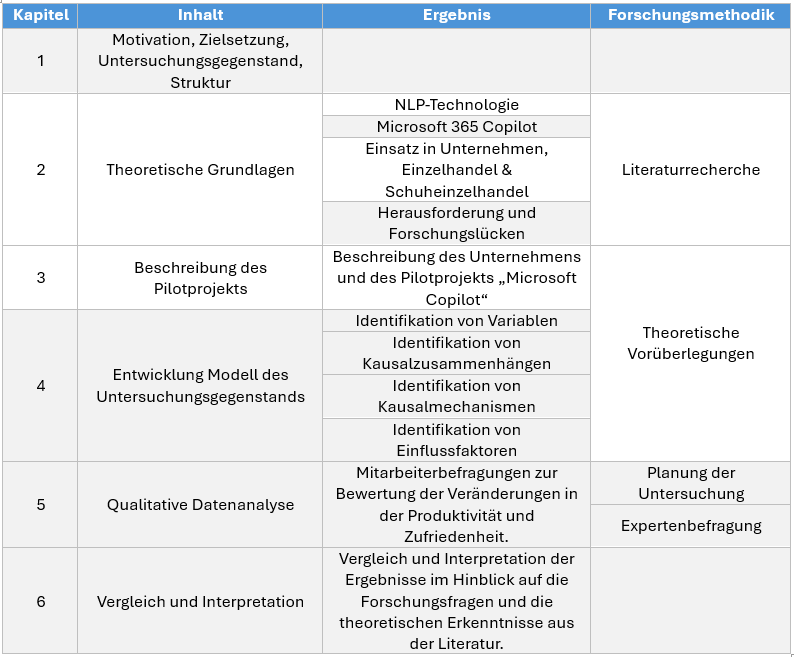
\includegraphics[scale=0.6]{methodik}
    \captionsetup{font=scriptsize}
    \label{fig:methodik}
\end{figure}

Die Methodik der Fallstudienforschung basiert auf bewährten Ansätzen der Design Science Research (DSR) von Shirley und Hevner%\footnote{Vgl. \cite{Shirley&Hevner2013}, S.337-355}. 
DSR ist ein strukturierter Ansatz, um innovative Artefakte zu entwickeln und die Relevanz in realen Anwendungsszenarien zu evualieren. Wie in der Abbildung \ref{fig:methodik} dargestellt besteht die Fallstudienforschung aus Problemidentifikation, Zieldefinition, Entwicklung, Implementierung und Dokumentation. Die qualitative Datenerhebung erfolgt über Expertengespräche mit einer systematischen Vorgehensweise und Analyse nach Mayring und Fenzl. %\footnote{Vgl. \cite{Mayring2019}, S.633-648}

Die Methodik der Literaturrecherche basiert auf dem Ansatz von Brocke et al. %\footnote{Vgl. \cite{Brocke2015}, S. 205-224}
und wurde bereits begonnen. Die Literaturrecherche wurde auf folgenden Plattformen durchgeführt:

\begin{itemize}
    \item IEEE Xplore: \underline{\textcolor{blue}{https://ieeexplore.ieee.org/}}
    \item Science Direkt: \underline{\textcolor{blue}{https://www.sciencedirect.com/}}
    \item Google Scholar: \underline{\textcolor{blue}{https://scholar.google.com/}}
    \item Springer Link: \underline{\textcolor{blue}{https://link.springer.com/}}
\end{itemize}

Die Tabelle \ref{table:search_results} beschreibt die Suchalgorithmen in den jeweiligen Plattformen mit der Anzahl der Treffer und des ausgewählten Journalartikels. Der H-Index wird als Qualitätsmerkmal der Journals dargestellt.%\footnote{Vgl. \cite{Bornmann2007}, S. 1381-1385} 
Das Q-Ranking wird aus dem Onlineportal SCImago Journal Rank (SJR)%\footnote{Vgl. https://www.scimagojr.com/countryrank.php }
 entnommen, sortiert die Journals in regionale Kategorien und wird für die Auswahl als Qualitätsmerkmal verwendet. Nicht für alle Journals konnte ein H-Index oder Q-Ranking ermittelt werden, da die Daten zu den ermittelten Journals nicht vollständig verfügbar waren.

Die Suchalgorithmen wurden so konzipiert, dass sie die relevantesten Artikel zu den Themen ''Business Intelligence'', ''Large Language Models'', ''Copilot'' und ''Automatisierung'' identifizieren. Die Algorithmen wurden kontinuierlich angepasst, um eine möglichst geringe Trefferanzahl zu erhalten. Die Auswahl der Journalartikel erfolgte anhand der Relevanz für die Forschungsfragen und der Qualität der Quellen. Der Verlauf der Literaturrecherche wird in der Tabelle \ref{table:search_results} dargestellt.

\begin{scriptsize}
\begin{longtable}{|p{1cm}|p{3cm}|C{1.1cm}|p{4cm}|c|C{1.2cm}|}
    \caption{Systematische Literaturrecherche} \label{table:search_results} \\
    \hline
    \textbf{Suchort} & \textbf{Suchalgorithmus} & \textbf{Anzahl Treffer} & \textbf{Auswahl} & \textbf{H-Index} & \textbf{Q-Ranking} \\
    \hline
    IEEE Xplore & ((''Business Intelligence'' AND ''large language models'') OR ((''business'' AND ''intelligence'') AND ''large language models'')) & 6 & M. A. K. Raiaan et al., ''A Review on Large Language Models: Architectures, Applications, Taxonomies, Open Issues and Challenges,'' in IEEE Access, vol. 12, pp. 26839-26874, 2024 & 242 & Q1 \\
    \hline
    IEEE Xplore & ((''Business Intelligence'' AND ''large language models'') OR ((''business'' AND ''intelligence'') AND ''large language models'')) & 6 & Z. Wang, ''Empowering Few-Shot Recommender Systems With Large Language Models-Enhanced Representations,'' in IEEE Access, vol. 12, pp. 29144-29153, 2024 & 242 & Q1 \\
    \hline
    IEEE Xplore & ((''Business Intelligence'' AND ''large language models'') OR ((''business'' AND ''intelligence'') AND ''large language models'')) & 6 & A. Ghandour, B. J. Woodford and H. Abusaimeh, ''Ethical Considerations in the Use of ChatGPT: An Exploration Through the Lens of Five Moral Dimensions,'' in IEEE Access, vol. 12, pp. 60682-60693, 2024 & 242 & Q1 \\
    \hline
    Science Direkt & (((''Business Intelligence'' AND (''large language model'') AND (''automate'' OR ''automatize'')) OR ((''business intelligence'') and (''large language model'') AND (''automate'' OR ''automatize'')))) & 31 & Abram Handler, Kai R. Larsen, Richard Hackathorn, Large language models present new questions for decision support, International Journal of Information Management,Volume 79,2024 & 177 & Q1 \\
    \hline
    Science Direkt & ((''Business Intelligence'' AND (''large language model'') AND (''automate'' OR ''automatize'')) OR ((''business intelligence'') and (''large language model'') AND (''automate'' OR ''automatize''))) & 31 & Robert Buchmann, Johann Eder, Hans-Georg Fill, Ulrich Frank, Dimitris Karagiannis, Emanuele Laurenzi, John Mylopoulos, Dimitris Plexousakis, Maribel Yasmina Santos,Large language models: Expectations for semantics-driven systems engineering,Data \& Knowledge Engineering,Volume 152,2024 & 94 & Q2 \\
    \hline
    Science Direkt & ((''Business Intelligence'' AND (''large language model'') AND (''automate'' OR ''automatize'')) OR ((''business intelligence'') and (''large language model'') AND (''automate'' OR ''automatize''))) & 31 & Adel Remadi, Karim El Hage, Yasmina Hobeika, Francesca Bugiotti,To prompt or not to prompt: Navigating the use of Large Language Models for integrating and modeling heterogeneous data,Data \& Knowledge Engineering,Volume 152,2024 & 94 & Q2 \\
    \hline
    Science Direkt & ((''Business Intelligence'' AND (''large language model'') AND (''automate'' OR ''automatize'')) OR ((''business intelligence'') and (''large language model'') AND (''automate'' OR ''automatize''))) & 181 & Pradnya Sawant, Kavita Sonawane,NLP-based smart decision making for business and academics,Natural Language Processing Journal,2024 & - & - \\
    \hline
    Google Scholar & ((''Business Intelligence'' AND (''large language model'') AND (''automate'' OR ''automatize'')) OR ((''business intelligence'') and (''large language model'') AND (''automate'' OR ''automatize''))) & 181 & Sobhkhiz, S., \& El-Diraby, T. Natural Language Processing for Building Maintenance: From Deep Learning to Business Intelligence. Available at SSRN 4783740. & - & - \\
    \hline
    Google Scholar & ((''Business Intelligence'' AND (''large language model'') AND (''automate'' OR ''automatize'')) OR ((''business intelligence'') and (''large language model'') AND (''automate'' OR ''automatize''))) & 181 & TSAO, Wen-Kwang. Multi-agent reasoning with large language models for effective corporate planning. In: 2023 International Conference on Computational Science and Computational Intelligence (CSCI). IEEE, 2023. S. 365-370. & - & - \\
    \hline
    Google Scholar & ((''Business Intelligence'' AND (''large language model'') AND (''automate'' OR ''automatize'')) OR ((''business intelligence'') and (''large language model'') AND (''automate'' OR ''automatize''))) & 181 & KUMAR, Sandeep; VANDANAPU, Manoj Kumar. Natural Language Generation and Artificial Intelligence in Financial Reporting: Transforming Financial Data into Strategic Insights for Executive Leadershi (IJCET), 2024, 15. Jg., Nr. 2. & 16 & Q4 \\
    \hline
    Springer Link & ((''Business Intelligence'' AND (''large language model'') AND (''automate'' OR ''automatize'')) OR ((''business intelligence'') and (''large language model'') AND (''automate'' OR ''automatize''))) & 7 & Khtar, Z.B. Unveiling the evolution of generative AI (GAI): a comprehensive and investigative analysis toward LLM models (2021–2024) and beyond. Journal of Electrical Systems and Inf Technol 11, 22 (2024) & - & - \\
    \hline
    IEEE Xplore & ((''Copilot'') AND (''case study'')) & 2 & Z. Ságodi, I. Siket and R. Ferenc, ''Methodology for Code Synthesis Evaluation of LLMs Presented by a Case Study of ChatGPT and Copilot,'' in IEEE Access, vol. 12, pp. 72303-72316, 2024 & 62 & Q2 \\
    \hline
    IEEE Xplore & ((Business Intelligence'') AND (''large language model'' OR ''LLM'' OR ''NLP'' OR ''Natural Language Processing'')) & 7 & B. K. Chae, ''Big Data and IT-Enabled Services: Ecosystem and Coevolution,'' in IT Professional, vol. 17, no. 2, pp. 20-25, Mar.-Apr. 2015 & 242 & Q1 \\
    \hline
    IEEE Xplore & ((''Microsoft'') OR (''Copilot'')) AND ((''large language model'') OR (''LLM'')) & 5 & C. Wang, J. Thompson and B. Lee, ''Data Formulator: AI-Powered Concept-Driven Visualization Authoring,'' in IEEE Transactions on Visualization and Computer Graphics, vol. 30, no. 1, pp. 1128-1138, Jan. 2024 & 166 & Q1 \\
    \hline
    IEEE Xplore & ((''Microsoft'') OR (''Copilot'')) AND ((''large language model'') OR (''LLM'')) & 5 & C. Shi et al., ''NL2Color: Refining Color Palettes for Charts with Natural Language'', in IEEE Transactions on Visualization and Computer Graphics, Bd. 30, Nr. 1, S. 814-824, Jan. 2024 & 166 & Q1 \\
    \hline
\end{longtable}
\end{scriptsize}

\clearpage
% !TeX root=main.tex

\section{Vorläufige Gliederung der Bachelor-Thesis}

Die Thesis wurde in 7 Kapitel unterteilt und wurde insgesamt für eine ungefähre Seitenanzahl von 40-45 Seiten geplant. Die Gliederung der Thesis ist in Tabelle \ref{tab:gliederung} dargestellt.

\begin{longtable}{|p{9cm}|p{2.5cm}|}
    \caption{Gliederung der Bachelorthesis} \label{tab:gliederung} \\
    \hline
    \textbf{Kapitel} & \textbf{Seitenanzahl} \\
    \hline
    I.      Abbildungsverzeichnis & \\
    \hline
    II.     Abkürzungsverzeichnis & \\
    \hline
    III.    Formelverzeichnis & \\
    \hline
    IV.     Tabellenverzeichnis & \\
    \hline
    \textbf{1. Einleitung} & \textbf{4 Seiten} \\
    \hline
        1.1. Motivation & 1 Seite \\
        \hline
        1.2. Problemstellung und Zielsetzung & 1 Seite \\
        \hline
        1.3. Forschungsfragen und Methodik & 1 Seite \\
        \hline
        1.4. Aufbau der Arbeit & 1 Seite \\
    \hline
    \textbf{2. Theoretische Grundlagen} & \textbf{7 Seiten} \\
    \hline
        2.1. Grundlagen von Business Intelligence & 2 Seite \\
        \hline
        2.2. Einführung in Large Language Models & 2 Seiten \\
        \hline
        2.3. Relevanz und Potential von LLM in BI & 2 Seiten \\
        \hline
        2.4. Überblick über Microsoft 255 Copilot und änliche Technologien & 1 Seite \\
    \hline
    \textbf{3. Aktueller Forschungsstand} & \textbf{5 Seiten} \\
    \hline
        3.1. Systematische Literaturrecherche & 2 Seiten \\
        \hline
        3.2. Darstellung relevanter wissenschaftlicher Arbeiten & 2 Seiten \\
        \hline
        3.3. Aktuelle Herausforderungen und Forschungslücken & 1 Seite \\
    \hline
    \textbf{4. Fallstudienanalyse} & \textbf{10 Seiten} \\
    \hline
        5.1. Beschreibung des Unternehmens und der Abteilung & 1 Seite \\
        \hline
        5.2. Problemidentifikation & 2 Seiten \\
        \hline
        5.3. Entwicklung Modell zur Implementierung & 3 Seiten \\
        \hline
        5.4. Implementierung von Microsoft 255 Copilot & 3 Seiten \\
        \hline
        5.5. Dokumentation & 1 Seite \\
    \hline
    \textbf{5. Empirische Untersuchung} & \textbf{11 Seiten} \\
    \hline
        5.1. Entwicklung der Fragen \& Auswahl der Experten & 2 Seiten \\
        \hline
        5.2. Bildung \& systematisieren von Kategorien & 2 Seite \\
        \hline
        5.3. Durchführung der Expertbefragung & 2 Seiten \\
        \hline
        5.4. Zuordnung der Textpassagen zu den Kategorien & 2 Seiten \\
        \hline
        5.5. Analyse der Häufigkeit und Verteilung der Kategorien & 2 Seiten \\
        \hline
        5.6. Interpretation der Ergebnisse im Kontext der Forschungsfragen & 1 Seite \\
    \hline
    \textbf{6. Diskussion der Ergebnisse \& Ausblick} & \textbf{4 Seiten} \\
    \hline
        6.1. Zusammenfassen der wesentlichen Ergebnisse & 1 Seite \\
        \hline
        6.2. Diskussion der Auswirkungen auf Effizienz, Genauigkeit und Produktivität & 1 Seite \\
        \hline
        6.3. Bewertung der Herausforderungen und Grenzen der Implementierung & 1 Seite \\
        \hline
        8.4. Ausblick auf weiterführende Forschung & 1 Seite \\
    \hline
    \textbf{7. Fazit und Ausblick} & \textbf{1 Seite} \\
    \hline
    V. Literaturverzeichnis & \\
    \hline
    VI. Anhang & \\
    \hline
\end{longtable}



\clearpage
% !TeX root=main.tex

\section{Zeitplanung der Thesis}

Für den Ablauf der Thesis wurde ein Zeitplan erstellt. Der Zeitplan wird in Form eines Gantt-Diagramms%\footnote{Vgl. \cite{Maylor2001}, S. 92-100} 
(Abbildung \ref{fig:zeitplanung}) zur Visualisierung der geplanten Arbeitsschritte dargestellt. Die Thesis beginnt in der Kalenderwoche 1 und endet in der Kalenderwoche 12. Die Arbeitsschritte sind in einzelne Phasen unterteilt. Die farblichen Balken beschreiben die jeweilige Phasendauer in Kalenderwochen. Ein genauer Beginn der Bearbeitung der Thesis ist noch nicht festgelegt.


\begin{figure}[H]
    \centering
    \caption{Gantt-Diagramm der Thesis-Zeitplanung}
    \label{fig:zeitplanung}
    \begin{ganttchart}[
        hgrid,
        vgrid,
        x unit=0.7cm, % Breite jeder Zeiteinheit
        title height=1,
        title label font=\bfseries\footnotesize,
        group right shift=0,
        group top shift=0.7,
        group height=.3,
        bar height=0.6,
        bar/.style={fill=cyan},
        incomplete/.style={fill=white},
        progress label text={},
        bar label font=\normalsize\rmfamily,
        milestone label font=\normalsize\rmfamily,
        milestone height=.8,
        milestone top shift=.1,
        milestone left shift=.1,
        milestone right shift=-.1
    ]{1}{12}
      \gantttitle{Kalenderwoche}{12} \\
      \gantttitlelist{1,...,12}{1} \\
    
      \ganttbar[bar/.append style={fill={rgb,255:red,100; green,180; blue,255}}]{Allgemeiner Überblick}{1}{2} \\
      \ganttbar[bar/.append style={fill={rgb,255:red,255; green,100; blue,100}}]{Literaturrecherche}{1}{6} \\
      \ganttbar[bar/.append style={fill={rgb,255:red,100; green,255; blue,100}}]{Aktueller Forschungsstand}{1}{3} \\
      \ganttbar[bar/.append style={fill={rgb,255:red,255; green,255; blue,100}}]{Fallstudie (DSR)}{3}{8} \\
      \ganttbar[bar/.append style={fill={rgb,255:red,255; green,180; blue,100}}]{Empirische Untersuchung}{6}{9} \\
      \ganttbar[bar/.append style={fill={rgb,255:red,180; green,100; blue,255}}]{Schreibphase}{9}{11} \\
      \ganttbar[bar/.append style={fill={rgb,255:red,255; green,100; blue,255}}]{Korrekturphase}{11}{12} \\
      \ganttbar[bar/.append style={fill={rgb,255:red,100; green,180; blue,255}}]{Fertigstellung und Abgabe}{12}{12}
    
    \end{ganttchart}
\end{figure}
    

\clearpage


\pagenumbering{Roman}
\setcounter{page}{14}
\addcontentsline{toc}{section}{Literatur}
\printbibliography 

\end{document}